\section{Active Filters}

The active filter operates creating waveforms to interact with the voltages and currents presented in the electrical grid to establish a power factor equal to one. This is accomplished by measuring the voltage waveforms from the power source and the current waveforms from the load, and then using these parameters on the instantaneous power theory to determine the current reference as an input to be set in a compensator. The compensator injects current waveforms in the circuit with symmetrical values of the components which degrades the power factor. The typical system compounded by a non-linear load with an active filter is presented in Fig. \ref{fig:compensador.png}.

\begin{figure}[!t]
\centering
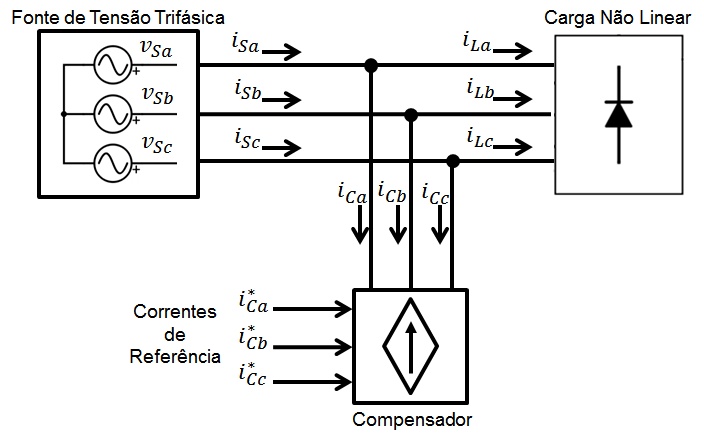
\includegraphics[width=2.8in]{Figures/compensador.png}
\caption{Simulation Results}
\label{fig_sim}
\end{figure}

%\begin{figure}
%	\centering
%	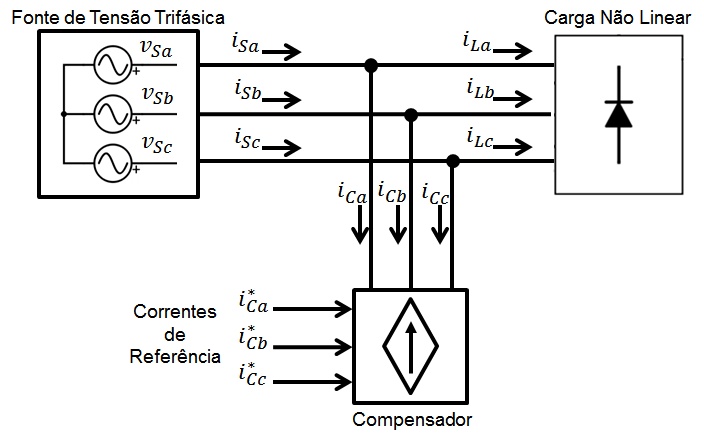
\includegraphics[width=0.4\textwidth]{Figures/compensador.png}
%	\caption{Simulation Results}
%	\label{fig:compensador.png}
%\end{figure}


\subsection{Instantaneous Power Theory}

The instantaneous power theory was presented by Akagi \cite{Akagi}, which proposed some new concepts for the instantaneous active and reactive power. This theory can be used in three phase, three or four wire system and in steady or transient state \cite{Akagi,Akagi}. In this theory, the manipulation of the active and reactive power calculations brings a tool to determine the currents that carry some content which degrade the power factor, such as harmonic distortion and phase shift.
Considering a three-phase system, composed by the phases $a$, $b$ and $c$, the instantaneous power theory is based in the coordinates transformation from the $abc$ to $\alpha \beta 0 $. This is known as the Clarke Transformation and is shown in eq. (2) \ref{eq:Clarke}.

\begin{equation}
\begin{aligned}
\begin{bmatrix}
v_0\\
v_\alpha\\
v_\beta
\end{bmatrix}
& = \sqrt{\dfrac{2}{3}}
\begin{bmatrix}
\dfrac{1}{\sqrt{2}}	& \dfrac{1}{\sqrt{2}}	& \dfrac{1}{\sqrt{2}}		\\[2ex]
1					& -\dfrac{1}{2}			& -\dfrac{1}{2}				\\[2ex]
0					& \dfrac{\sqrt{3}}{2}	& -\dfrac{\sqrt{3}}{2}
\end{bmatrix}
\begin{bmatrix}
v_a\\
v_b\\
v_c
\end{bmatrix}
;\\
\begin{bmatrix}
i_0\\
i_\alpha\\
i_\beta
\end{bmatrix}
& = \sqrt{\dfrac{2}{3}}
\begin{bmatrix}
\dfrac{1}{\sqrt{2}}	& \dfrac{1}{\sqrt{2}}	& \dfrac{1}{\sqrt{2}}		\\[2ex]
1					& -\dfrac{1}{2}			& -\dfrac{1}{2}				\\[2ex]
0					& \dfrac{\sqrt{3}}{2}	& -\dfrac{\sqrt{3}}{2}
\end{bmatrix}
\begin{bmatrix}
i_a\\
i_b\\
i_c
\end{bmatrix}
\label{eq:Clarke}
\end{aligned}
\end{equation} 

According to \cite{Akagi}, the instantaneous power is defined as shown in eq (3) \ref{eq:pq_0}, where the $p_0$, $p$ and $q$ are the instantaneous zero-sequence power, the active instantaneous power and the reactive instantaneous power, respectively \cite{Akagi,Peng1996}.

\begin{equation}
\begin{bmatrix}
p_0\\
p\\
q
\end{bmatrix}=
\begin{bmatrix}
v_0		&	0			&	0\\
0		&	v_{\alpha}	&	v_{\beta}\\
0		&	v_{\beta}	&	-v_{\alpha}
\end{bmatrix}
\begin{bmatrix}
i_{0}
i_{\alpha}\\
i_{\beta}
\end{bmatrix}
\label{eq:pq_0}
\end{equation} 

Considering a system without zero-sequence voltage and/or current, such as the aircraft electrical system, the eq (3) can be simplified as the eq (4), where the instantaneous zero-sequence power is absent.

\begin{equation}
\begin{bmatrix}
p\\
q
\end{bmatrix}=
\begin{bmatrix}
v_{\alpha}	&	v_{\beta}\\
v_{\beta}	&	-v_{\alpha}
\end{bmatrix}
\begin{bmatrix}
i_{\alpha}\\
i_{\beta}
\end{bmatrix}
\label{eq:pq}
\end{equation} 

The reverse calculation, i.e., the determination of the currents $i_{\alpha}$ and $i_{\beta}$ when the voltages $v_{alpha}$ and $v_{\beta}$ and the instantaneous power $p$ and $q$ are known is presented in eq. (5) \ref{eq:i_alphabeta}.

\begin{equation}
\begin{bmatrix}
i_{\alpha}\\
i_{\beta}
\end{bmatrix}=
\dfrac{1}{v_{\alpha}^2+v_{\beta}^2}
\begin{bmatrix}
v_{\alpha}	&	v_{\beta}\\
v_{\beta}	&	-v_{\alpha}
\end{bmatrix}
\begin{bmatrix}
p\\
q
\end{bmatrix}
\label{eq:i_alphabeta}
\end{equation}

By definition, the active instantaneous power is composed by the energy that is swapped between two subsystems, whereas the reactive power is composed by the energy being swapped between the 3 phases of the system \cite{Akagi}. Furthermore, both $p$ and $q$ can be defined as a composition of an average ($\overline{p}$ and $\overline{q}$) and an oscillating ($\tilde{p}$ and $\tilde{q}$) values, as defined in eq. (6) \ref{eq:pq_m_o}.

\begin{equation}
\begin{aligned}
p = \overline{p} + \tilde{p}\\
q = \overline{q} + \tilde{q} 
\end{aligned}
\label{eq:pq_m_o}
\end{equation} 

To create an active filter to coordinate a power factor equal to 1, the only permitted power flowing in the transmission lines is the average value of the instantaneous active power ($\overline{p}$). To ensure this condition, the filter must inject in the lines currents which contains the symmetrical values of the instantaneous reactive power ($q$) and the oscillating portion of the instantaneous active power ($\tilde{p}$) created by the non-linear load. By doing this, these powers are cancelled in the same way as the current harmonic content. Thereby, the selection of power to be compensate and processed by the filter must contains the values of the $-\tilde{p}$ and $-q$ only.

The filter full operation is defined by the instantaneous power $p$ and $q$ calculation, followed by the selection of the power to be compensated, i.e., $-\tilde{p}$ and $-q$. Afterwards, the currents $i_{\alpha}$ and $i_{\beta}$ are calculated using the eq (5) \ref{eq:i_alphabeta} with the values $-\tilde{p}$ and $-q$, followed by the inverse Clarke transformation to acquire the current in $abc$ coordinates to be applied as a reference in the compensator. The whole active filter reference definition is shown in Fig. \ref{fig:diagrama_filtro.png}.

\begin{figure}[!th]
	\centering
	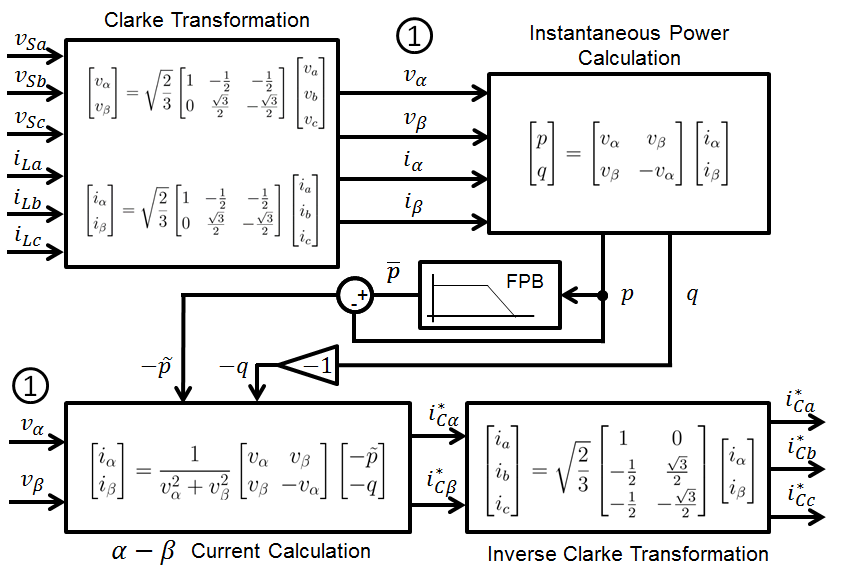
\includegraphics[width=3in]{Figures/diagrama_filtro.png}
	\caption{Simulation Results}
	\label{fig:diagrama_filtro.png}
\end{figure}

%\begin{figure}
%	\centering
%	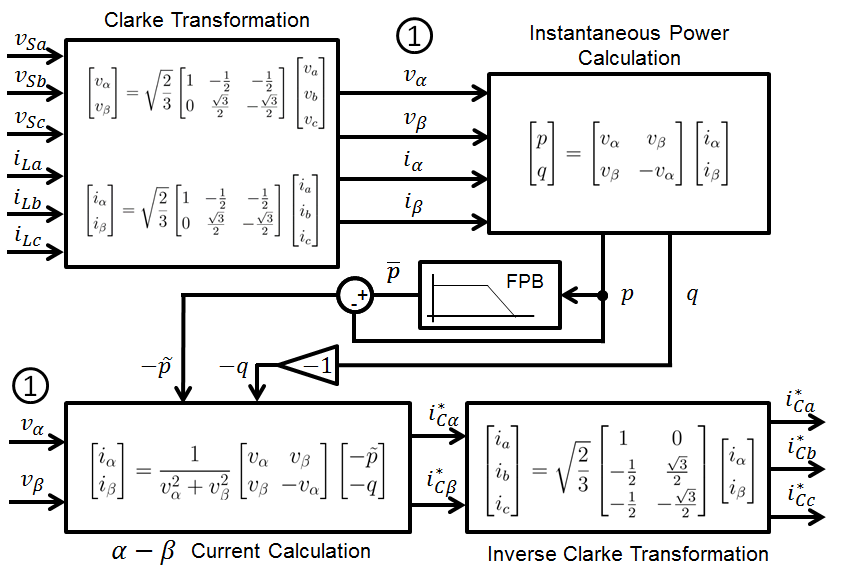
\includegraphics[width=0.47\textwidth]{Figures/diagrama_filtro.png}
%	\caption{Active filter reference definition}
%	\label{fig:diagrama_filtro.png}
%\end{figure}


\subsection{Control Strategy}

The active filter specified by the calculations procedure as defined in Fig (7) \ref{fig:diagrama_filtro.png} presents very effective to set the current reference to be applied in the compensator to mitigate the electrical system harmonic content. However, this calculation is valid to produce sinusoidal waveforms only when the voltages measured and used in the filter input is pure sinusoidal. This happen due to the filter operates allowing only the mean value of the active instantaneous power flowing in the circuit. Therefore, the use of a non-sinusoidal voltage waveform in the input of the filter cause the filter to creates a non-sinusoidal current waveform to order to establish the power flow without $q$ and $\tilde{p}$.

In aircraft electrical power system the voltage waveforms stated in the point of common connection (PCC) are presented as non-sinusoidal, but still limited by the aeronautical standards. As the voltages are measured at this point, the operation of the filter is not optimal for power quality purposes, and in some cases, might decrease the power quality and operates unstably depending the levels of harmonic distortion presented in the voltages waveforms.

According to \ cite {Akagi2007}, the p-q theory proves insufficient to satisfy the non-linear loads filtering in systems with previously distorted voltages waveforms and, at the same time, to satisfy the conditions of injecting a sinusoidal current and setting a flow of a constant flow active instantaneous power.  
 
\todo[inline]{Colocar os métodos de controle, focando no método de controle de corrente senoidal}
\todo[inline]{Falar do controle de tensão do capacitor (se couber, ou falar bem sucintamente)}

Descrição da sua proposta com detalhes. Método empregado para resolução do problema (equacionamento, pseudo código, diagrama de blocos etc.).
Caso utilize componentes específicos na implementação (circuito integrado, sensor etc.), não exagere na descrição dos mesmos (fotos, dados técnicos, especificação etc.). O leitor pode obter estes dados na referência que você indicou.	